\documentclass{xStandalone}

\begin{document}
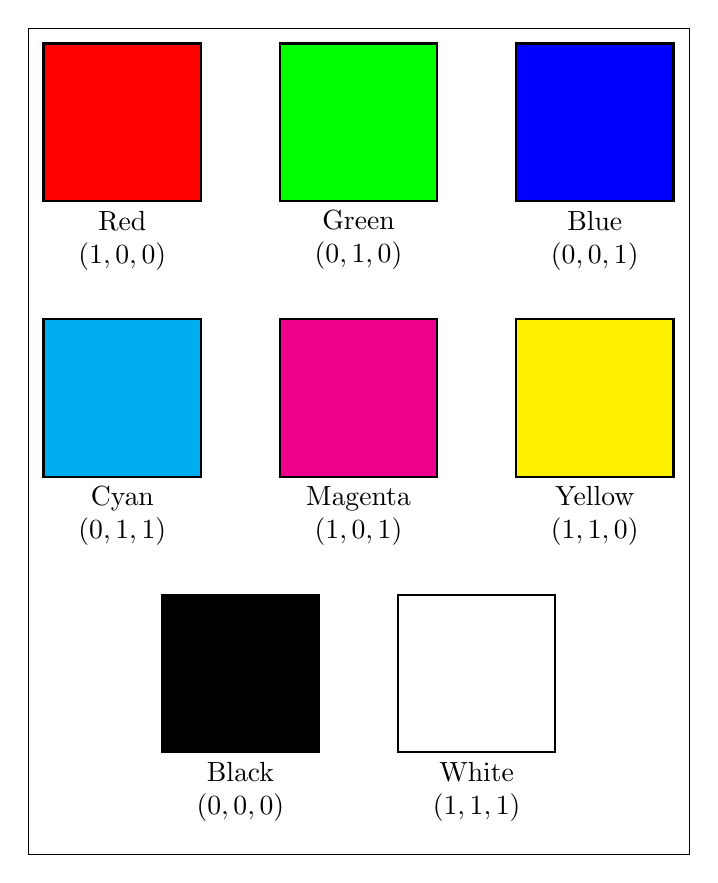
\begin{tikzpicture}

\draw[thick,fill=black] (1.5,0) rectangle ++ (2,2);
\draw[thick,fill=white] (4.5,0) rectangle ++ (2,2);

\draw[thick,fill=cyan] (0,3.5) rectangle ++ (2,2);
\draw[thick,fill=magenta] (3,3.5) rectangle ++ (2,2);
\draw[thick,fill=yellow] (6,3.5) rectangle ++ (2,2);

\draw[thick,fill=red] (0,7) rectangle ++ (2,2);
\draw[thick,fill=green] (3,7) rectangle ++ (2,2);
\draw[thick,fill=blue] (6,7) rectangle ++ (2,2);

\path (2.5,0) node[below,align=center] {Black\\ $(0,0,0)$};
\path (5.5,0) node[below,align=center] {White\\ $(1,1,1)$};

\path (1,3.5) node[below,align=center] {Cyan\\ $(0,1,1)$};
\path (4,3.5) node[below,align=center] {Magenta\\ $(1,0,1)$};
\path (7,3.5) node[below,align=center] {Yellow\\ $(1,1,0)$};

\path (1,7) node[below,align=center] {Red\\ $(1,0,0)$};
\path (4,7) node[below,align=center] {Green\\ $(0,1,0)$};
\path (7,7) node[below,align=center] {Blue\\ $(0,0,1)$};

\draw[ultra thin] (-0.2,-1.3) rectangle (8.2,9.2);

\end{tikzpicture}
\end{document}